%--------Sericio para la detección de comunidades
%--------Daniel Ochoa John
%--------20/07/2014
\newcolumntype{L}[1]{>{\raggedright\let\newline\\\arraybackslash\hspace{0pt}}m{#1}}
\newcolumntype{C}[1]{>{\centering\let\newline\\\arraybackslash\hspace{0pt}}m{#1}}
\newcolumntype{R}[1]{>{\raggedleft\let\newline\\\arraybackslash\hspace{0pt}}m{#1}}


\chapter{Servicio para la detección de comunidades}
\label{cap:servicio}

En este capítulo se describe el servicio de detección de comunidades que se desarrolló en este trabajo de tesis. En primer lugar, se caracteriza y describe a la arquitectura y sus componentes. Posteriormente, se declaran los algoritmos y \textit{endpoints} utilizados por el servicio. Finalmente, se muestra un ejemplo de funcionamiento con un problema clásico de la literatura.

\section{Caracterización del Servicio}

En la presente sección, se realiza una caracterización del servicio que se ha construido, desde un punto de vista, tanto tecnológico, en relación a aquellas herramientas desarrolladas para responsabilidades funcionales específicas e ingenieril, en relación a la combinación y comunicación de aquellas herramientas, para alcanzar un objetivo mayor.

\subsection{Descripción general}

Una de las principales dificultades de este trabajo de tesis ha sido la de añadir a RBox la capacidad de detectar comunidades de una manera limpia, es decir, sin afectar el funcionamiento actual del sistema. Esto implica que dicha añadidura no debe suponer, por una parte, una mayor reingeniería de los componentes que ya se han definido en la herramienta y por otra, una estricta dependencia de RBox con respecto al componente de detección de comunidades. En resumen, la nueva pieza de \textit{software} que se ha incorporado debe cumplir con los siguientes requisitos:

\begin{enumerate}[I]
  \item{No debe implicar modificaciones en el código de los componentes ya definidos.}
  \item{La pieza debe ser capaz de detectar comunidades.}
  \item{La pieza no debe impedir su reemplazo por otra con mayores prestaciones o mucho más específica.}
\end{enumerate}

Siguiendo estos tres principios básicos definidos para la aplicación, es que se ha tomado como alternativa una arquitectura orientada a servicios, ya que permite flexibilidad al integrarse con sistemas “legados” (Bianco, Kotermanski, & Merson, 2007).  Continuando con la misma línea de pensamiento, al momento de definir que tipo de servicio conviene disponibilizar, si un servicio Web SOAP\footnote{SOAP es el acrónimo de \textit{Simple Object Access Protocol}, que define un \textit{stack} de componentes para el intercambio de información entre aplicaciones.} convencional o un servicio de tipo REST\footnote{REST es el acrónimo de \textit{Representaton State Transfer}, que engloba y define una manera de acceder a recursos a través de la web únicamente utilizando el protocolo HTTP.}, se ha probado y evidenciado que los servicios de tipo REST son mayormente adecuados cuando se requieren integraciones estratégicas con otras aplicaciones, cuando el performance importa (Guinard, Ion, & Mayer, 2012). Luego, el servicio construido es de tipo REST.

Ahora bien, de las alternativas posibles para proveer un servicio que sea eficaz detectando comunidades: construir una librería con distintos algoritmos o seleccionar y adaptar una existente, se ha optado por la segunda alternativa, ya que existe una librería llamada igraph (Csárdi & Nepusz, 2006), construída bajo C, que provee diferentes estrategias y algoritmos típicamente utilizados para el análisis de grafos y en específico, la detección de comunidades. Esta librería cuenta con un encapsulamiento de la implementación en C hacia Python, lo que permite comunicar sus prestaciones con un \textit{framework} que soporte la construcción de servicios Web de tipo REST.

\subsection{Arquitectura del Servicio}

Como primer antecedente, y para contextualizar, es necesario mencionar la arquitectura que se ha definido para la construcción del servicio. La Figura \ref{fig:serv-im1} muestra un diagrama con los componentes definidos y sus interacciones. La descripción de cada uno de ellos es la siguiente:

\begin{itemize}
  \item \textbf{\textit{Client}:} es una aplicación, servicio o componente de \textit{software} que requiere un servicio de análisis de comunidades y, en concreto, un servicio de detección de comunidades. Este cliente debe preocuparse de encapsular la información de manera conveniente a la que el servicio espera al momento de realizar la petición de servicio, así como también de traducir la respuesta del recién mencionado. En el diagrama, esta situación se refleja como \textit{Wrapped Data}.
  \item \textbf{\textit{Network Environment}:} representa al ambiente de red que separa al cliente y al servicio. Es muy relevante considerarlo debido a que, dependiendo del tamaño del problema, es posible que el ambiente del cliente no requiera uno de alta disponibilidad de recursos (a.k.a \textit{cloud servers}). Sin embargo, el servicio puede abastecer a muchísimos clientes, por lo que puede requerir un ambiente escalable horizontalmente para su \textit{deployment}, como por ejemplo la nube de \textit{Amazon}.
  \item \textbf{Endpoints:} son las interfaces que expone el servicio para que los clientes se comunican con él. En el caso del servicio de detección de comunidades, cada \textit{endpoint} implica un algoritmo diferente para realizar la detección de comunidades.
  \item \textbf{Servicio:} el servicio es el resultado de la unión de distintas tecnologías. En primer lugar, y para permitir la exposición de un servicio Web de tipo rest, se utiliza flask-restful\footnote{Sitio web oficial en http://flask-restful.readthedocs.org/en/latest}. Luego, para permitir la comunicación con igraph, se utiliza un componente que encapsula la comunicación con la mencionada librería, llamada python-igraph. Finalmente, para todo el procesamiento y disponibilización de algoritmos, se utiliza la librería igraph. La especificación tanto de python-igraph como de igraph está disponible en el sitio Web oficial\footnote{Sitio web oficial de igraph para python en http://igraph.org/python/.}.
\end{itemize}

\begin{figure}
  \centering
  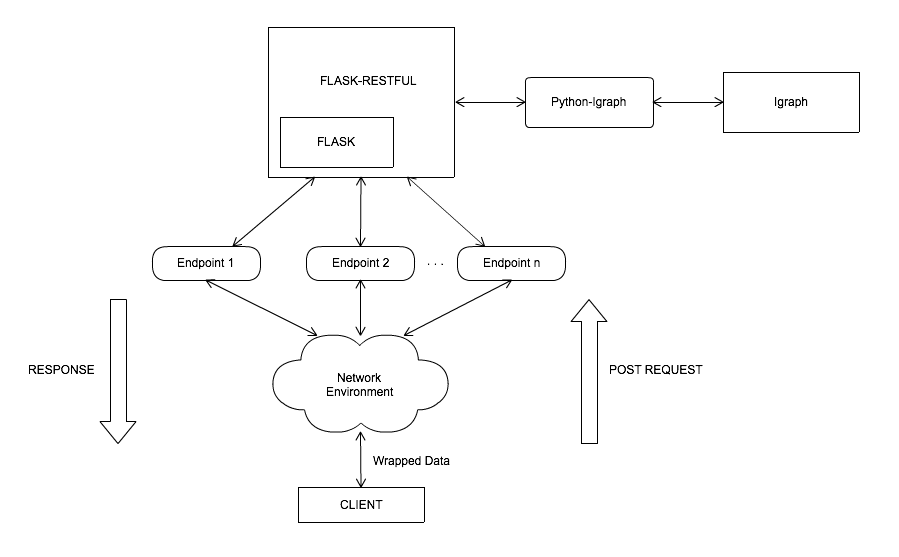
\includegraphics[scale=.5]{images/Figura3-1}
  \caption{\em Arquitectura del servicio de detección de comunidades.}
  \label{fig:serv-im1}
\end{figure}

\section{Algoritmos Utilizados}

En esta sección se enuncian los algoritmos que se han publicado mediante el servicio de detección de comunidades y que son aquellos que la librería igraph ha implementado. La Tabla \ref{tab:serv-tab01} muestra a cada uno de ellos y el endpoint en particular al que están sujetos.

\begin{enumerate}[I]
  \item \textbf{Multilevel} (Blondel, Guillaume, Lambiotte, \& Lefebvre, 2008): Maximización de la modularidad en donde los vecinos se juntan en comunidades, los cuales se juntan en comunidades de comunidades. En primer lugar, cada nodo se asigna a su propio módulo y luego cada nodo se mueve al módulo vecino que produzca el mayor aumento a la modularidad. Si no ocurre aumento alguno con ningún movimiento, entonces el nodo permanece en su módulo. Cada nodo puede ser considerado más de una vez. La red se reconstruye considerando a los módulos como nuevos nodos y se aplica el algoritmo nuevamente. Esto se repite hasta que la modularidad no puede ser maximizada.
  \item \textbf{Label Propagation} (Raghavan, Albert, \& Kumara, 2007): A cada uno de los nodos de un grafo se le asigna una marca o label. El procedimiento continúa iterativamente y a cada nodo se le asigna la marca mas frecuente de sus vecinos de una manera síncrona. El método se detiene cuando la marca de cada nodo es una de las marcas más frecuentes en su cluster o barrio. Es muy rápido, no obstante es no determinista.
  \item \textbf{Leading Eigenvector} (Newman, 2006): Enfoque jerárquico que optimiza la función de la modularidad. En cada iteración, el grafo se divide en dos partes de manera que se produzca un aumento en la modularidad. La separación está determinada mediante un vector principal de modularidad (eigenvector) y existe una condición de término que impide que los grupos que están densamente conectados se separen.
  \item \textbf{Infomap} (Rosvall \& Bergstrom, 2008): Minimización de una ecuación que describe la cantidad de movimientos de un camino aleatorio en una red jerárquica. Sigue la filosofía del método de Louvain: los vecinos se juntan en módulos, los cuales se juntan en super-módulos. Cada nodo se asigna a su propio módulo y luego, de manera aleatoria, cada nodo se mueve al módulo vecino que produzca la mayor reducción de la ecuación. Si no ocurre reducción alguna con ningún movimiento, entonces el nodo permanece en su módulo. Ahora, la red se reconstruye considerando a los módulos como nuevos nodos y se aplica el algoritmo nuevamente. Hasta que la ecuación ya no pueda ser minimizada.
  \item \textbf{Spinglass} (Traag \& Bruggeman, 2009): Enfoque desde la física estadística. En este modelo cada nodo es considerado una partícula y puede estar en uno de los estados de spin. Las interacciones entre las partículas, las aristas, especifican quienes prefieren tener el mismo estado de spin y quienes prefieren cambiarlo. El modelo se simula para un número definido de iteraciones y el spin de las partículas determina quienes son una comunidad. Este método es no determinista.
\end{enumerate}

\begin{table}
  \begin{center}
    \caption[Estrategias utilizadas para la detección de comunidades.]{Estrategias utilizadas para la detección de comunidades.}
    \label{tab:serv-tab01}
      \begin{tabular}{|L{6cm}|L{5cm}|}
        \hline
        \textbf{Algoritmo} & \textbf{Endpoint (POST)}\\ \hline
         \textit{Multilevel} &  /CommunityDetection/Multilevel \\ \hline
         \textit{Label Propagation} & /CommunityDetection/LabelPropagation \\ \hline
         Leading Eigenvector & /CommunityDetection/LeadingEigenvector \\ \hline
         Infomap  & /CommunityDetection/Infomap \\ \hline
         Spinglass & /CommunityDetection/Spinglass \\ \hline
      \end{tabular}
  \end{center}
\end{table}

\section{Ejemplo de Funcionamiento}

En esta sección se muestra el funcionamiento del servicio de detección de comunidades a partir de un ejemplo clásico en la literatura, que es detectar las comunidades en el club de karate de Zachary (Zachary, 1977), que tiene 34 nodos, 78 aristas y el máximo componente conectado es de 34 nodos. Para esto, se han destinado endpoints (ver Tabla \ref{tab:serv-tab02})  del servicio de manera tal que el ejemplo sea parte de la aplicación:

\begin{table}[H]
  \begin{center}
    \caption[Servicios que implementan el manejo de la detección de comunidades en el Club de Karate de Zachary.]{Servicios que implementan el manejo de la detección de comunidades en el Club de Karate de Zachary.}
    \label{tab:serv-tab02}
      \begin{tabular}{|L{6cm}|L{10cm}|}
        \hline
        \textbf{Descripción} & \textbf{Endpoint (GET)}\\ \hline
         JSON que representa el grafo del problema del club de karate de Zachary. & /KarateClub \\ \hline
         JSON que representa a las comunidades detectadas en el \textit{data\textit{set}} del club de karate de Zachary utilizando el mismo algoritmo que el \textit{endpoint} /CommunityDetection/\textit{Multilevel}. & /KarateClub/Communities/\textit{Multilevel} \\ \hline
         JSON que representa a las comunidades detectadas en el \textit{data\textit{set}} del club de karate de Zachary utilizando el mismo algoritmo que el \textit{endpoint} /CommunityDetection/LabelPropagation & /KarateClub/Communities/LabelPropagation \\ \hline
         JSON que representa a las comunidades detectadas en el \textit{data\textit{set}} del club de karate de Zachary utilizando el mismo algoritmo que el \textit{endpoint} /CommunityDetection/LeadingEigenvector & /KarateClub/Communities/LeadingEigenvector \\ \hline
         JSON que representa a las comunidades detectadas en el \textit{data\textit{set}} del club de karate de Zachary utilizando el mismo algoritmo que el \textit{endpoint} /CommunityDetection/Infomap & /KarateClub/Communities/Infomap \\ \hline
         JSON que representa a las comunidades detectadas en el \textit{data\textit{set}} del club de karate de Zachary utilizando el mismo algoritmo que el \textit{endpoint} /CommunityDetection/Spinglass & /KarateClub/Communities/Spinglass \\ \hline
      \end{tabular}
  \end{center}
\end{table}

La Figura \ref{fig:serv-im2} muestra el grafo que se genera al realizar el \textit{parsing} correspondiente luego de hacer el \textit{request} a /KarateClub. Cuando se realiza el \textit{request} a /KarateClub/Communities para detectar las comunidades que existen en el \textit{data\textit{set}} de Zachary el resultado, para cada algoritmo, se muestra desde la Figura \ref{fig:serv-im3} hasta la Figura \ref{fig:serv-im7}. La Tablas \ref{tab:serv-tab03} a \ref{tab:serv-tab07} describen las comunidades detectadas por extensión, para cada algoritmo:

\begin{figure}
  \centering
  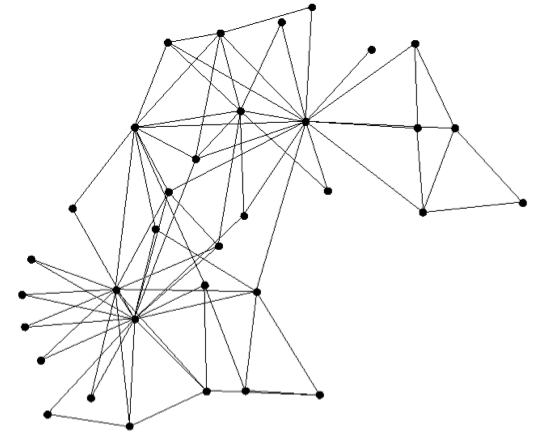
\includegraphics[scale=.6]{images/Figura3-2}
  \caption{\em Grafo que representa al Club de Karate de Zachary.}
  \label{fig:serv-im2}
\end{figure}

\begin{figure}[H]
  \centering
  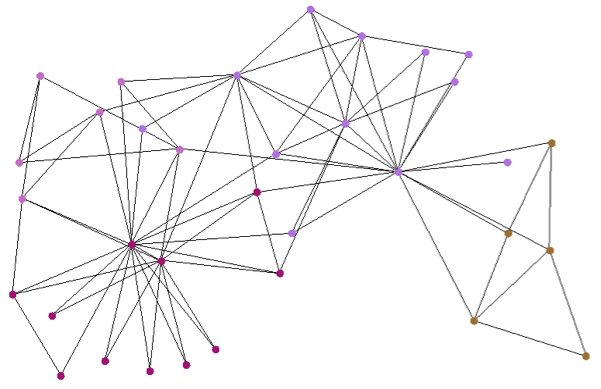
\includegraphics[scale=.6]{images/Figura3-3}
  \caption{\em Comunidades detectadas en el Club de Karate mediante el método \textit{\textit{Multilevel}}.}
  \label{fig:serv-im3}
\end{figure}

\begin{table}[H]
  \begin{center}
    \caption{Definición por extensión de las comunidades detectadas en el Club de Karate mediante el método \textit{\textit{Multilevel}}.}
    \label{tab:serv-tab03}
      \begin{tabular}{|L{4cm}|L{10cm}|}
        \hline
        \textbf{Nº Comunidad} & \textbf{Nodos}\\ \hline
         1 & 5, 6, 7, 11, 17 \\ \hline
         2 & 1, 2, 3, 4, 8, 10, 12, 13, 14, 18, 20, 22 \\ \hline
         3 & 24, 25, 26, 28, 29, 32 \\ \hline
         4 & 9, 15, 16, 19, 21, 23, 27, 30, 31, 33, 34 \\ \hline
      \end{tabular}
  \end{center}
\end{table}

\begin{figure}[H]
  \centering
  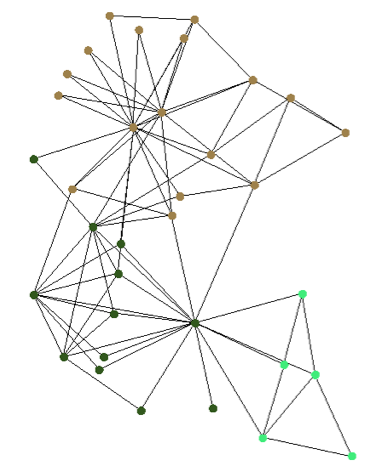
\includegraphics[scale=.6]{images/Figura3-4}
  \caption{\em Comunidades detectadas en el Club de Karate mediante una ejecución del método \textit{Label Propagation}.}
  \label{fig:serv-im4}
\end{figure}

\begin{table}[H]
  \begin{center}
    \caption{Definición por extensión de las comunidades detectadas en el Club de Karate mediante una ejecución del método \textit{Label Propagation}.}
    \label{tab:serv-tab04}
      \begin{tabular}{|L{4cm}|L{10cm}|}
        \hline
        \textbf{Nº Comunidad} & \textbf{Nodos}\\ \hline
         1 & 1, 2, 3, 4, 8, 10, 12, 13, 14, 18, 20, 22 \\ \hline
         2 & 5, 6, 7, 11, 17 \\ \hline
         3 & 9, 15, 16, 19, 21, 23, 24, 25, 26, 27, 28, 29, 30, 31, 32, 33, 34 \\ \hline
      \end{tabular}
  \end{center}
\end{table}

\begin{figure}[H]
  \centering
  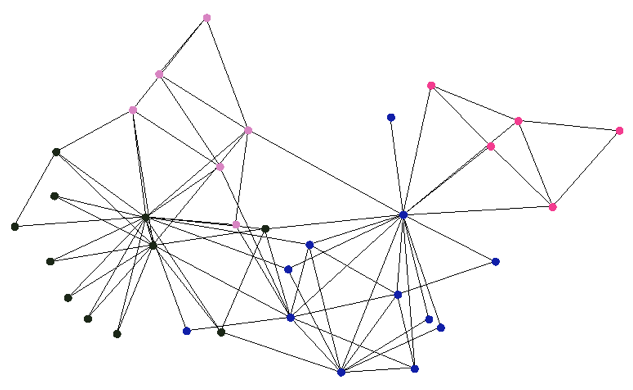
\includegraphics[scale=.6]{images/Figura3-5}
  \caption{\em Comunidades detectadas en el Club de Karate mediante el método \textit{Spinglass}.}
  \label{fig:serv-im5}
\end{figure}

\begin{table}[H]
  \begin{center}
    \caption{Definición por extensión de las comunidades detectadas en el Club de Karate mediante el método \textit{Spinglass}.}
    \label{tab:serv-tab05}
      \begin{tabular}{|L{4cm}|L{10cm}|}
        \hline
        \textbf{Nº Comunidad} & \textbf{Nodos}\\ \hline
         1 & 24, 25, 26, 28, 29, 32 \\ \hline
         2 & 5, 6, 7, 11, 17 \\ \hline
         3 & 1, 2, 3, 4, 8, 10, 12, 13, 14, 18, 20, 22 \\ \hline
         4 & 9, 15, 16, 19, 21, 23, 27, 30, 31, 33, 34 \\ \hline
      \end{tabular}
  \end{center}
\end{table}

\begin{figure}[H]
  \centering
  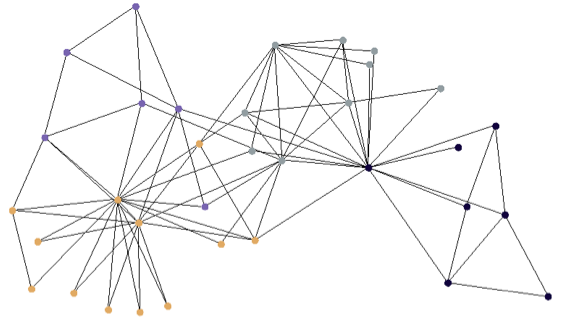
\includegraphics[scale=.6]{images/Figura3-6}
  \caption{\em Comunidades detectadas en el Club de Karate mediante el método \textit{LeadingEigenvector}.}
  \label{fig:serv-im6}
\end{figure}

\begin{table}[H]
  \begin{center}
    \caption{Definición por extensión de las comunidades detectadas en el Club de Karate mediante el método \textit{LeadingEigenvector}.}
    \label{tab:serv-tab06}
      \begin{tabular}{|L{4cm}|L{10cm}|}
        \hline
        \textbf{Nº Comunidad} & \textbf{Nodos}\\ \hline
         1 & 1, 5, 6, 7, 11, 12, 17 \\ \hline
         2 & 9, 10, 15, 16, 19, 21, 23, 27, 30, 31, 33, 34 \\ \hline
         3 & 2, 3, 4, 8, 13, 14, 18, 20, 22 \\ \hline
         4 & 24, 25, 26, 28, 29, 32 \\ \hline
      \end{tabular}
  \end{center}
\end{table}

\begin{figure}[H]
  \centering
  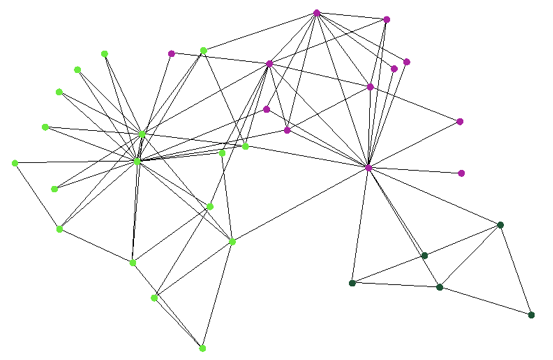
\includegraphics[scale=.6]{images/Figura3-7}
  \caption{\em Comunidades detectadas en el Club de Karate mediante el método \textit{Infomap}.}
  \label{fig:serv-im7}
\end{figure}

\begin{table}[H]
  \begin{center}
    \caption{Definición por extensión de las comunidades detectadas en el Club de Karate mediante el método \textit{Infomap}.}
    \label{tab:serv-tab07}
      \begin{tabular}{|L{4cm}|L{10cm}|}
        \hline
        \textbf{Nº Comunidad} & \textbf{Nodos}\\ \hline
         1 & 1, 2, 3, 4, 8, 10, 12, 13, 14, 18, 20, 22 \\ \hline
         2 & 5, 6, 7, 11, 17 \\ \hline
         3 & 9, 15, 16, 19, 21, 23, 24, 25, 26, 27, 28, 29, 30, 31, 32, 33, 34 \\ \hline
      \end{tabular}
  \end{center}
\end{table}

\section{Resumen}

En este capítulo se presentó el servicio de detección de comunidades que se utilizará RBox. Se han descrito los fundamentos mediante los cuales se tomó la decisión de seleccionar tecnologías y componentes. Posteriormente, se ha descrito la arquitectura del servicio componente a componente. Finalmente, se han enunciado los \textit{endpoints} que proveerá el servicio y, mediante un ejemplo, se ha mostrado su funcionamiento detectando comunidades para un mismo \textit{data\textit{set}} y con distintos algoritmos.
